\documentclass[cn,11pt,twocol]{elegantbook-zh-tw}

\usepackage{blindtext}

\title{生物統計 (Biostatistics)}
\subtitle{課堂講義}

\author{施銘杰}
\institute{清華大學學士後醫學系}
\date{\today}
\version{0.01}

% \extrainfo{Far better an approximate answer to the right question, which is often vague, than an exact answer to the wrong question, which can always be made precise. --- J. Tukey}

\extrainfo{}

\logo{NTHU.png}
\cover{cover.jpg}

\begin{document}
\maketitle
\tableofcontents
\mainmatter
\hypersetup{pageanchor=true}

\chapter{統計學概論}
    在這個資料取得越來越容易的時代,各個領域都希望能夠分析手上的資料、獲得結論並進行決策。例如在醫療領域中,我們常想知道一個療法對於病患的預後是否有影響,以進行後續補助政策的制定或治療指引的撰寫;或是能不能夠利用病患的影像資料、抽血資料和病史預測疾病的發生率,以達到提前篩檢、早期診斷、早期治療的目的。因此,如何有效率地整理資料、去蕪存菁、並進行合乎科學原理的分析便變成為一門顯學。統計便是一門利用科學方法來處理並分析資料的學科。當今因為資訊計算能力的超指數成長,分析整理資料的方法種類和複雜度也呈現爆炸性的增長,但這些方法的目的仍然是探尋資料內部隱含的資訊,因此背後仍然是以統計架構為基石。本課程前半段將著重統計觀念的建立,包含為什麼需要利用統計方法分析資料,以及推論統計的邏輯基礎。後半段則將介紹常用的統計檢定與迴歸方法,並輔以因果推論的理論框架介紹,以期了解如何針對有興趣的研究議題,選擇適當的統計模型並解讀分析結果。在本章,我們會簡介統計學的發展歷史,並帶出統計學的兩大分支:描述性和推論性統計。針對推論性統計,我們還會探討母體、抽樣和樣本的概念,以及這些概念如何融合到推論性統計的流程中。

\begin{introduction}[第 \thechapter 章學習目標]
    \item 描述性統計和推論性統計的目的
    \item 母體、樣本和抽樣的概念
    \item 推論性統計的流程與背後假設
    \item 統計推論的初步評讀
\end{introduction}

\section{統計的分支:敘述性統計}
    相較於其他領域,統計是一門十分近代才成型的學科,約十八世紀才開始發展。統計的英文是 \textit{statistics},拉丁字源為 \textit{statisticum},意謂「政府的」,因為統計最初是政府用來處理國家級資料(例如人口、經濟),以幫助管理國家的方法。首度將 \textit{statistics} 這個字引入英文的人據傳是蘇格蘭的 Sir John Sinclair (1754-1835)。他編纂了一本共有 22 集的 \textit{Statistical Account of Scotland},記錄了當時蘇格蘭當時的各式資料,包括地理、人口、農工生產等等,且紀錄內容並不限於數字。例如圖\ref{fig:john_sinclair}所示,書中內容記錄了其中一個地區的人口職業分佈,還提到當地的道路狀況。

\begin{figure}[htbp]
  \centering
  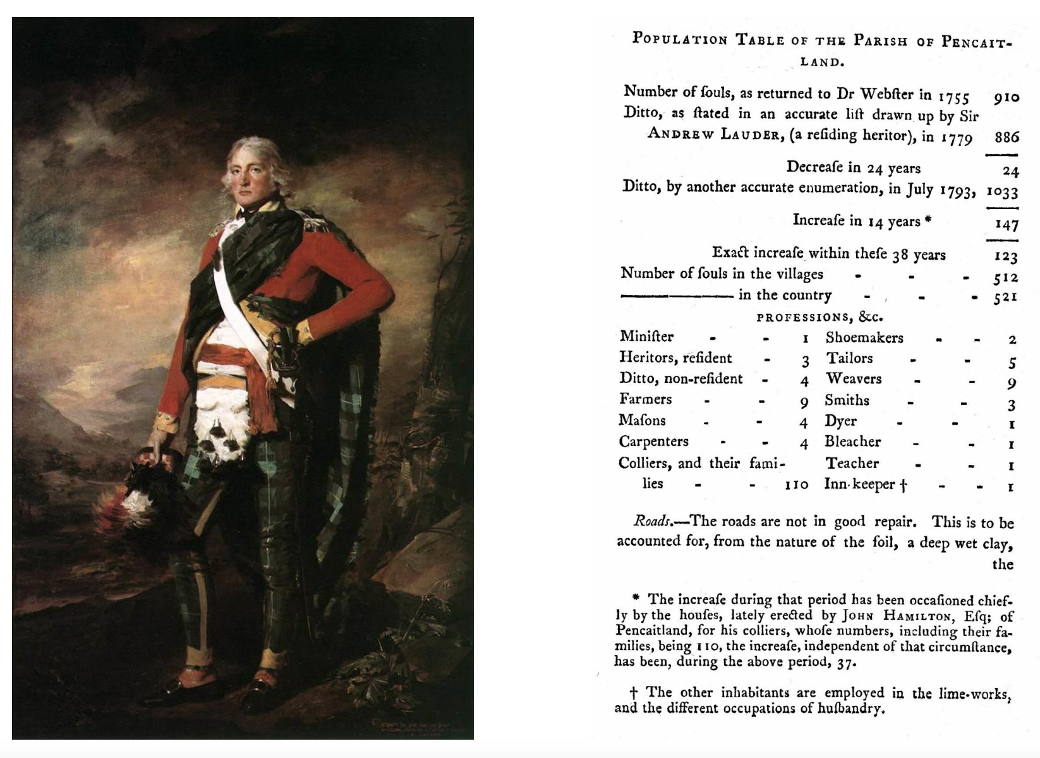
\includegraphics[width=0.9\textwidth]{figures/01-Overview/john_sinclair.png}
  \caption{Sir John Sinclair (1754-1835) 與 \textit{Statistical Account of Scotland} 的內頁}
  \label{fig:john_sinclair}
\end{figure}

    類似 \textit{Statistical Account of Scotland} 這類將資料整理後,以易懂的圖表呈現的方式一般被稱為\textit{描述性統計} (descriptive statistics)。描述統計學能將相對大量的資料精簡為具有代表性的統計數據(例如比例、平均值、中位數等描述統計量)或是圖片,以幫助我們快速了解資料的特性與隱含的訊息。運用得當的描述統計方法能夠讓決策者根據資料帶來的訊息即時地做出決策。例如,1854 年倫敦蘇活區 (Soho) 霍亂大爆發。該時代對於霍亂的病原為何仍然莫衷一是,但內科醫師 John Snow (1813-1858) 猜想霍亂的病原可能來自於水,因此根據蘇活區霍亂病例在家戶的分布做了圖 \ref{fig:john_snow},其中同一家戶的病例數越多,長條圖就越長。John Snow 發現霍亂病例似乎有以圖中的紅點為中心群聚分佈的趨勢,而該紅點標記的是蘇活區的一個公用抽水幫浦,和 John Snow 猜想的水媒傳染相符合。當地市政府而後也決定將抽水幫浦的手柄移除。John Snow 則因一系列霍亂相關的研究而被譽為「流行病學之父」。從這個圖片可以看出,John Snow將病例用散佈圖的方式標記是明智之舉。如果單純調查各分區的病例數而未作圖,則不見得能發現地理位置的群聚現象。

    \begin{figure}[htbp]
      \centering
      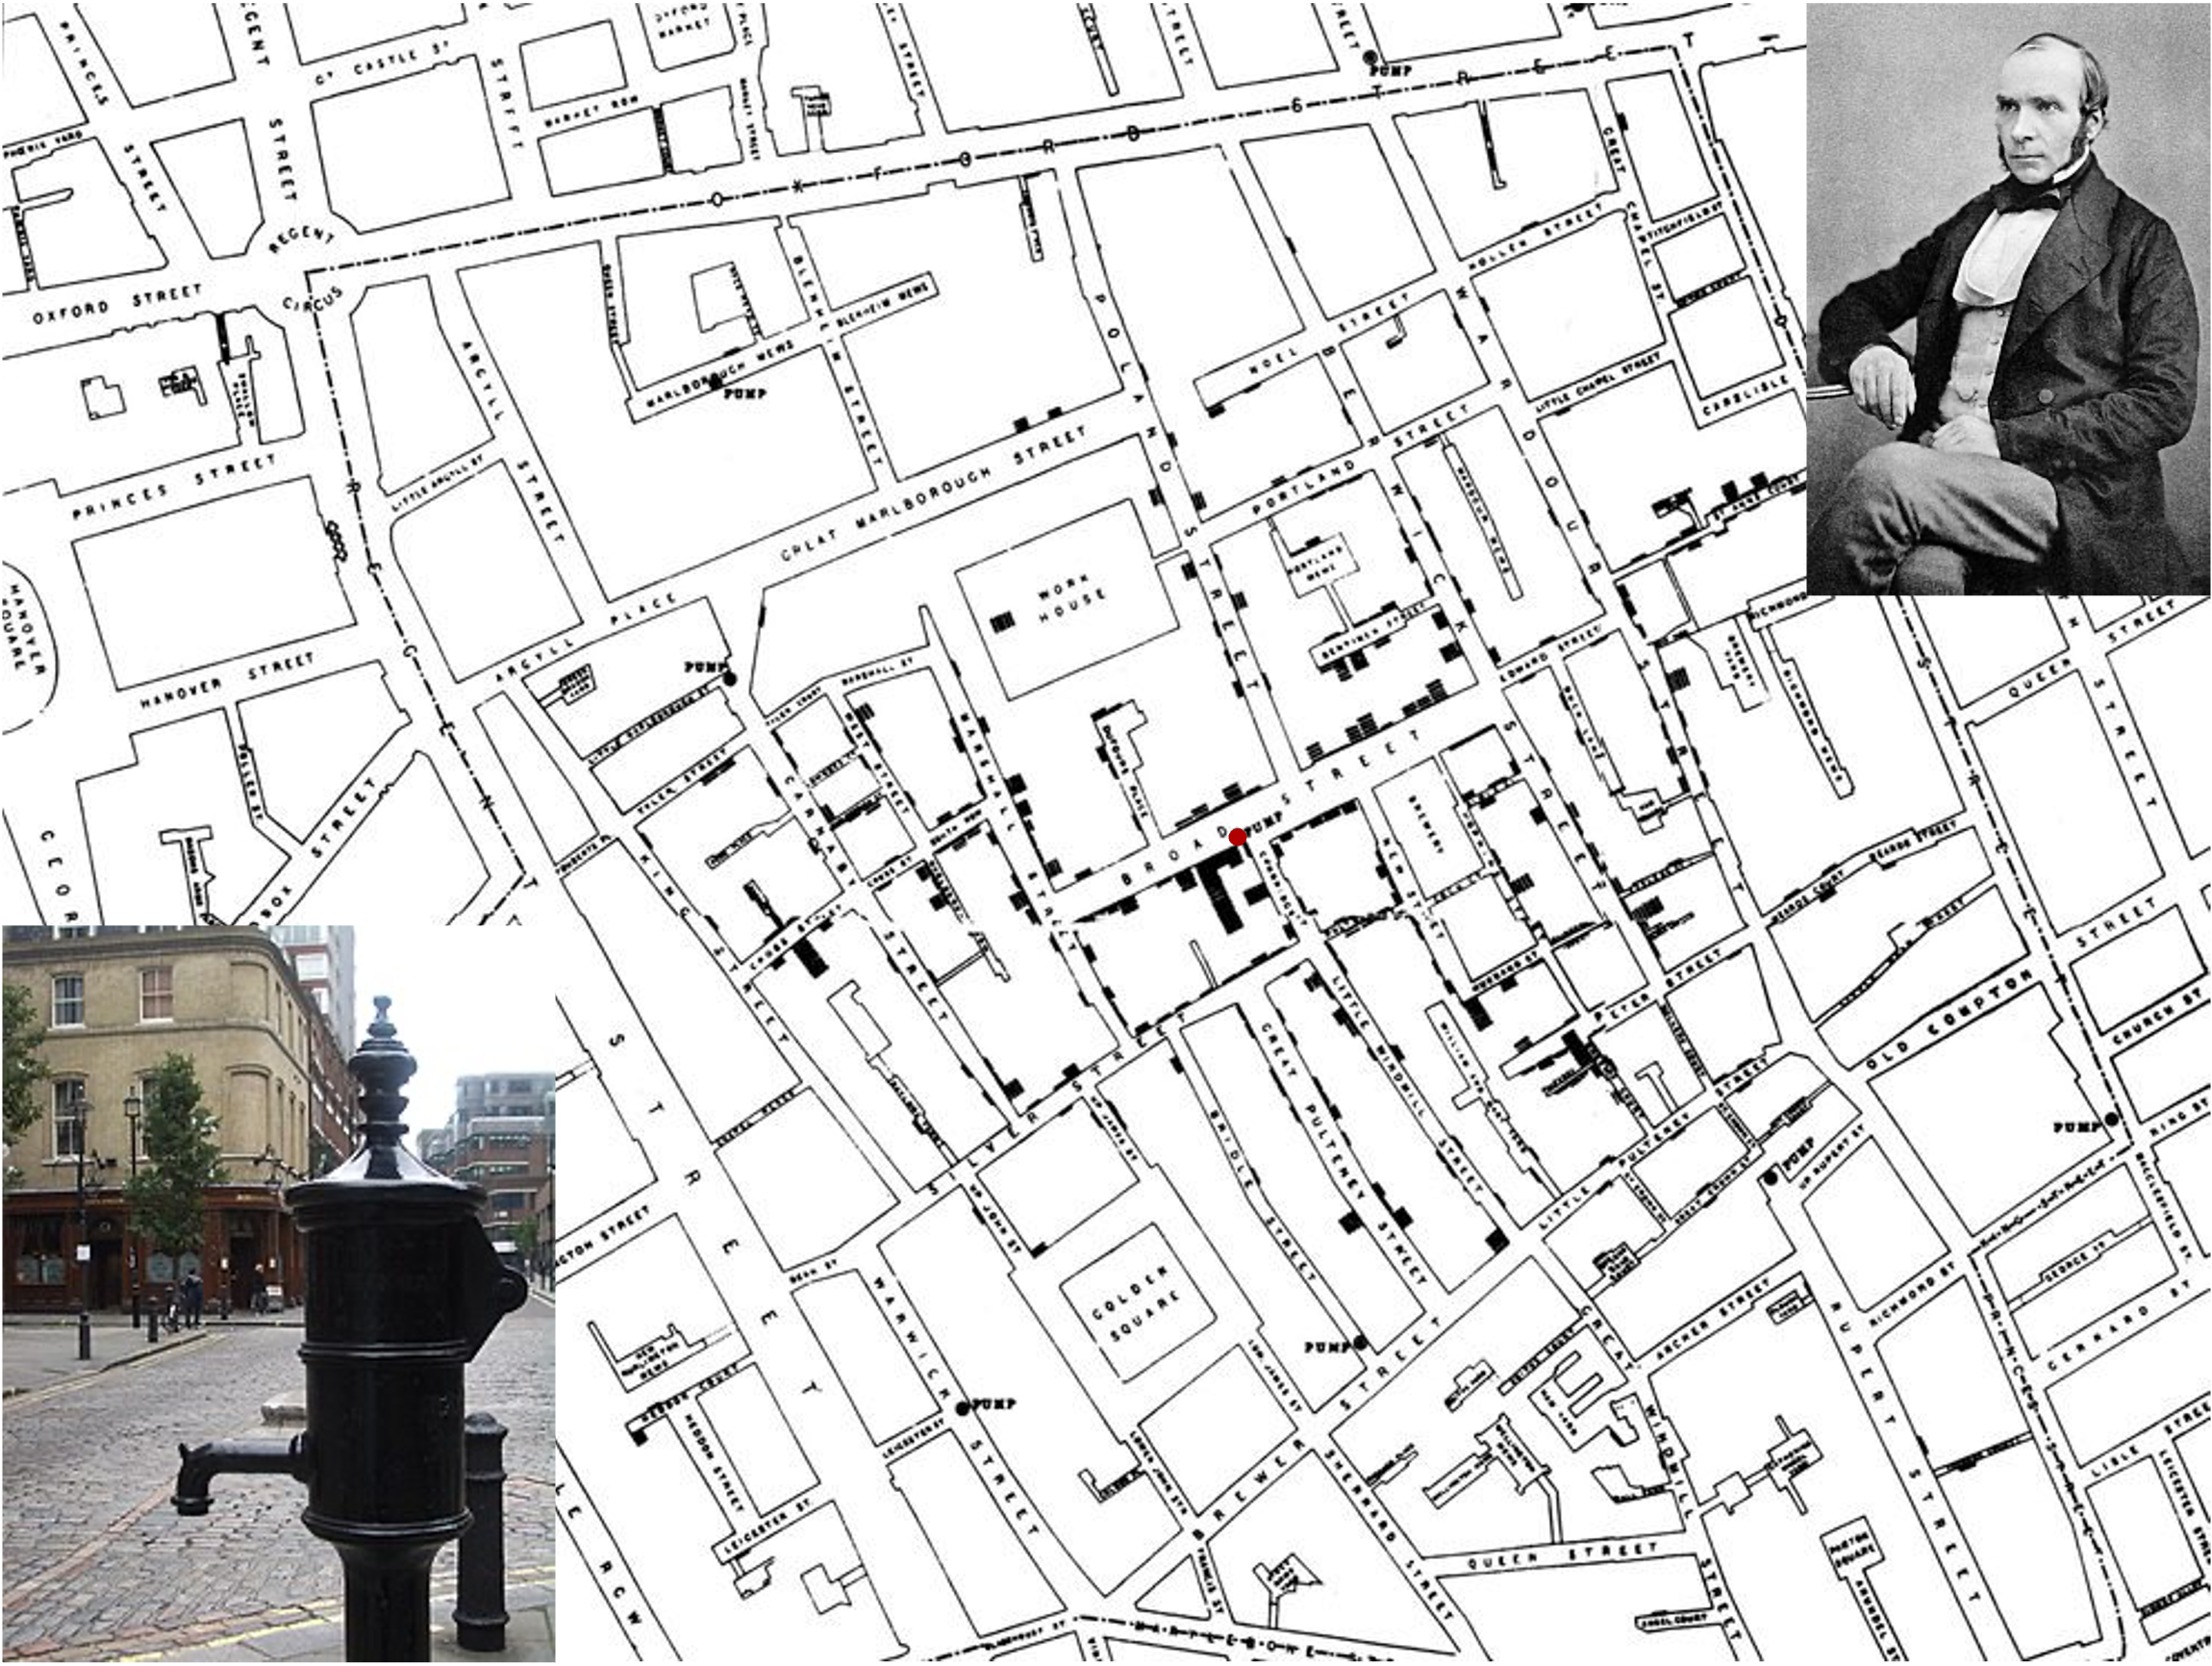
\includegraphics[width=0.9\textwidth]{figures/01-Overview/john_snow.png}
      \caption{John Snow (1813-1858)、其繪製的霍亂地圖、及地圖中心的公用抽水幫浦}
      \label{fig:john_snow}
    \end{figure}
    
    \bigskip
    
    \begin{custom}{思考}
        從 John Snow 繪製的圖片,是否已經足夠證明水就是霍亂的傳播根源?後來市政府將抽水幫浦的手柄移除,同時間霍亂疫情也逐漸緩和,如此是否已經足夠證明水就是霍亂的傳播根源?
    \end{custom}
    
    \bigskip
    
\section{統計的分支:推論性統計}

    有了描述統計學後,決策者理論上即可根據圖像或描述統計量來做決策。例如,利用健保資料庫了解國人糖尿病的患病率後,即可用患病率這個描述統計量估算糖尿病相關照護計畫的預算。然而,很多時候因為資源的限制,我們沒有辦法針對有興趣的目標量取得所有的資料。例如,如果我們有一個針對小細胞肺癌的新藥,並想要了解當前台灣第三期肺癌的病人服用該藥的副作用發生率(我們簡寫為 $p$)如何。理想上,我們想要搜集所有第三期肺癌的病人,都給予新藥後,評估出現副作用的比例。然而,這樣的作法在金錢資源上和倫理上都行不通。
    
    針對這個問題,一個可行的替代方法是,我們可以募集 $50$ 位第三期肺癌的病人,並給予新藥後,評估這 $50$ 位病人出現副作用發生率。比方說有 $2$ 位出現副作用,因此這群病人的副作用發生率為 $4\%$。只要我們募集的病人具有代表性,那麼「當前台灣第三期肺癌病人」的副作用發生率 $p$ 應該會和這群病人類似,大約是 $4\%$。然而,$p$ 顯然不太可能剛剛好是 $4\%$,因為這個算出來的 $4\%$ 會隨著募集到的病患不同而變動:如果重新募集另外兩組 $50$ 位病人,發生副作用的人數可能因為隨機性而變成 $1$ 人或 $3$ 人,進而算得 $2\%$ 或 $6\%$ 的發生率。因此,我們只知道 $p$ 應該在 $4\%$ 左右,但是它的實際數值則因為隨機的變動而有不確定性。因此,統計學家引進了數學的機率論來描述並處理不確定性,因而衍生出\textit{推論性統計}(Inferential statistics)。
    
    在推論性統計中,有幾個名詞是我們必須需要熟悉的。我們條列如下,並以上述例子作為對照:

    \begin{itemize}
        \item \textit{母體} (Population):我們實際上有興趣的總群體,「當前台灣第三期肺癌的病人」。
        \item \textit{參數} (Parameter):我們有興趣的目標量,「肺癌病人接受新藥的副作用發生率 $p$」。
        \item \textit{抽樣} (Sampling):從母體抽取一部份個體的過程。
        \item \textit{樣本} (Sample):從母體抽出的個體,「$50$ 人的第三期肺癌病人」。
        \item \textit{樣本數} (Sample size):樣本的個體數,「$50$」。
        \item \textit{參數估計式} (Parameter estimator):根據我們對母體的假設及抽樣方法,建構出一個估計參數的方法,「樣本中發生副作用的人數除以樣本數」。
        \item \textit{參數估計量} (Parameter estimate):把樣本帶入參數估計式得到的數值,「$4\%$」。
    \end{itemize}

    隨後,根據圖\ref{fig:flowchart}的流程,我們可以利用推論性統計的技巧,根據抽樣方法和母體假設對參數做推論,例如「當前台灣第三期肺癌病人服用新藥的副作用發生率 $95\%$ 信賴區間為 $(0.49\% - 13.71\%)$」或「在 $5\%$ 的顯著水準下,沒有足夠證據顯示當前台灣第三期肺癌病人服用新藥的副作用發生率大於 $1\%$」等等。以上的推論現在看起來可能不知所云,但後續課程將詳細介紹推論性統計的解讀方法,而後我們就會知道這些推論背後的意義,以及為什麼要弄得那麼複雜。
    
    圖\ref{fig:flowchart}的流程也給我們一個檢視統計推論中每個環節是否正確的藍圖。例如,針對公共議題的民意調查,如果只在火車站或夜市附近作隨機街訪,則樣本來源都只來自活動於火車站或夜市附近的居民,因而可能無法我們預想的「全民」母體。針對心血管疾病發病率的預測模型,如果建模資料來自於高階健檢的檢查資料,則該預測模型可能無法外推到全國國民使用。進行氣喘急性發作危險因子的分析時,如果單一病患因多次發作而提供多筆資料,但是使用的分析方法卻假設抽樣得到的樣本是互不相關,那麼得到的推論結果就會有偏誤。而且我們可以看到,推論統計中數學能夠做的只是根據母體假設以及抽樣方法儘量建構好的參數估計方法,但如果母體假設有誤或抽樣流程不正確,那麼統計能夠幫忙的程度就非常有限。
    
    \begin{figure}[htbp]
      \centering
      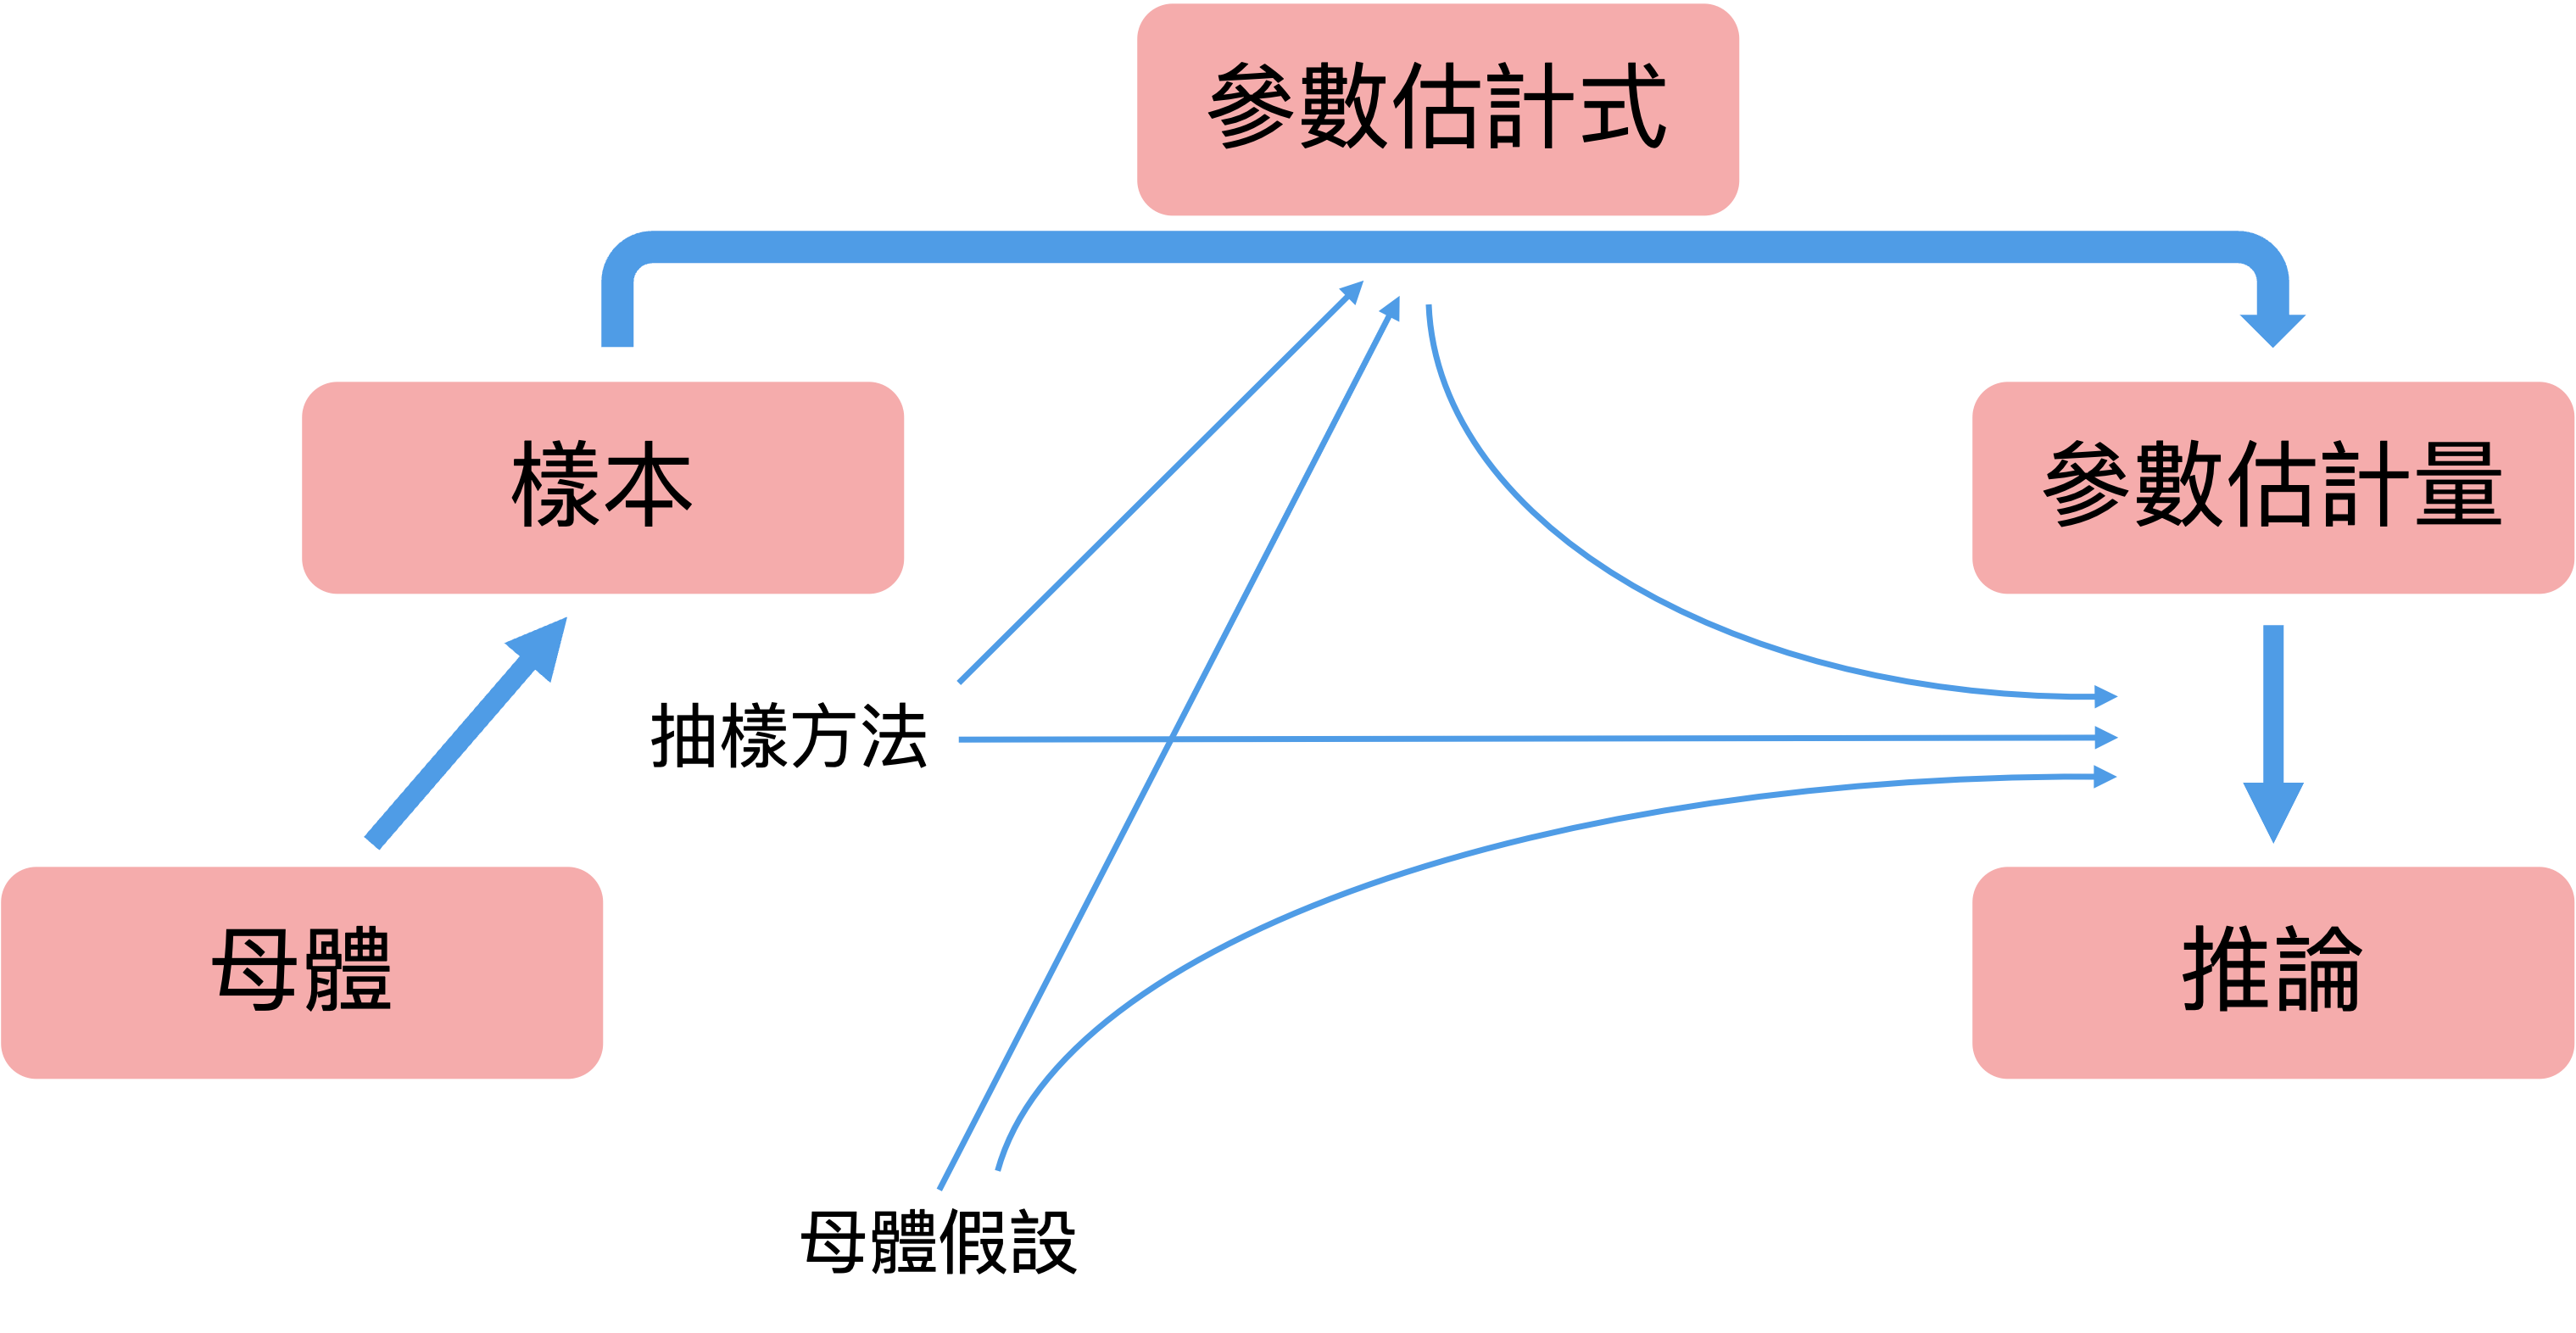
\includegraphics[width=0.9\textwidth]{figures/01-Overview/flowchart.png}
      \caption{推論統計的流程架構}
      \label{fig:flowchart}
    \end{figure}
    
    \bigskip
    
    \begin{custom}{思考}
        現今健保資料庫的覆蓋率已經超過 99.7\%。如果以台灣民眾為母體,那麼健保資料庫等同幾乎收集了母體的所有資料。在這個情況下,還有推論統計的必要嗎?
    \end{custom}
    
    \bigskip
    
    \begin{custom}{思考}
        在問卷調查中(例如:調查對某政策的支持與否),經常會出現某些題目漏答或拒答的現象。此時如果是以下的假設情境,是不是能夠用有回答的問卷估計出正確的政策支持率?(1) 漏(拒)答是完全隨機的,和受訪者的任何特性均無關;(2) 漏(拒)答不是完全隨機的,且和受訪者支不支持政策有關;(3) 漏(拒)答並非完全隨機,但僅和受訪者的性別、年齡有關,且問卷中有詢問性別及年齡;(4) 漏(拒)答並非完全隨機,但僅和受訪者的教育程度有關,但問卷未詢問教育程度。
    \end{custom}
    
\section{統計學的獨立發展}

    統計學的雛型雖然從十八世紀萌芽,並接受數學機率論的薰陶而逐漸茁壯,但直到十九世紀末,統計學才作為一門獨立、有系統性的學門發展。其中最重要的推手是研究遺傳學的 Francis Galton (1822-1911) 以及他的門生 Karl Pearson (1857-1936)。Galton 受到他的堂哥、也是遺傳學家的 Charles Darwin 的影響,對於連續性狀如身高、智力的遺傳感興趣。Galton 試圖用數學模型來分析並描述這些性狀的遺傳特性,因而發展出了回歸、相關性等等統計學最基本的概念。Pearson 作為 Galton 的門生(及被贊助者),完善了回歸及相關性的數學架構,並提出了假設檢定、卡方檢定、主成分分析等等統計方法與工具。而後,Ronald Fisher (1890-1962) 大力推進了遺傳以及推論統計的數學理論,並基於農業研究提出實驗設計法以及其統計分析,如變異數分析 (analysis of variance)。Galton、Pearson 和 Fisher 三人為當代推論性統計打下了重要基礎。
    
    \begin{figure}[htbp]
      \centering
      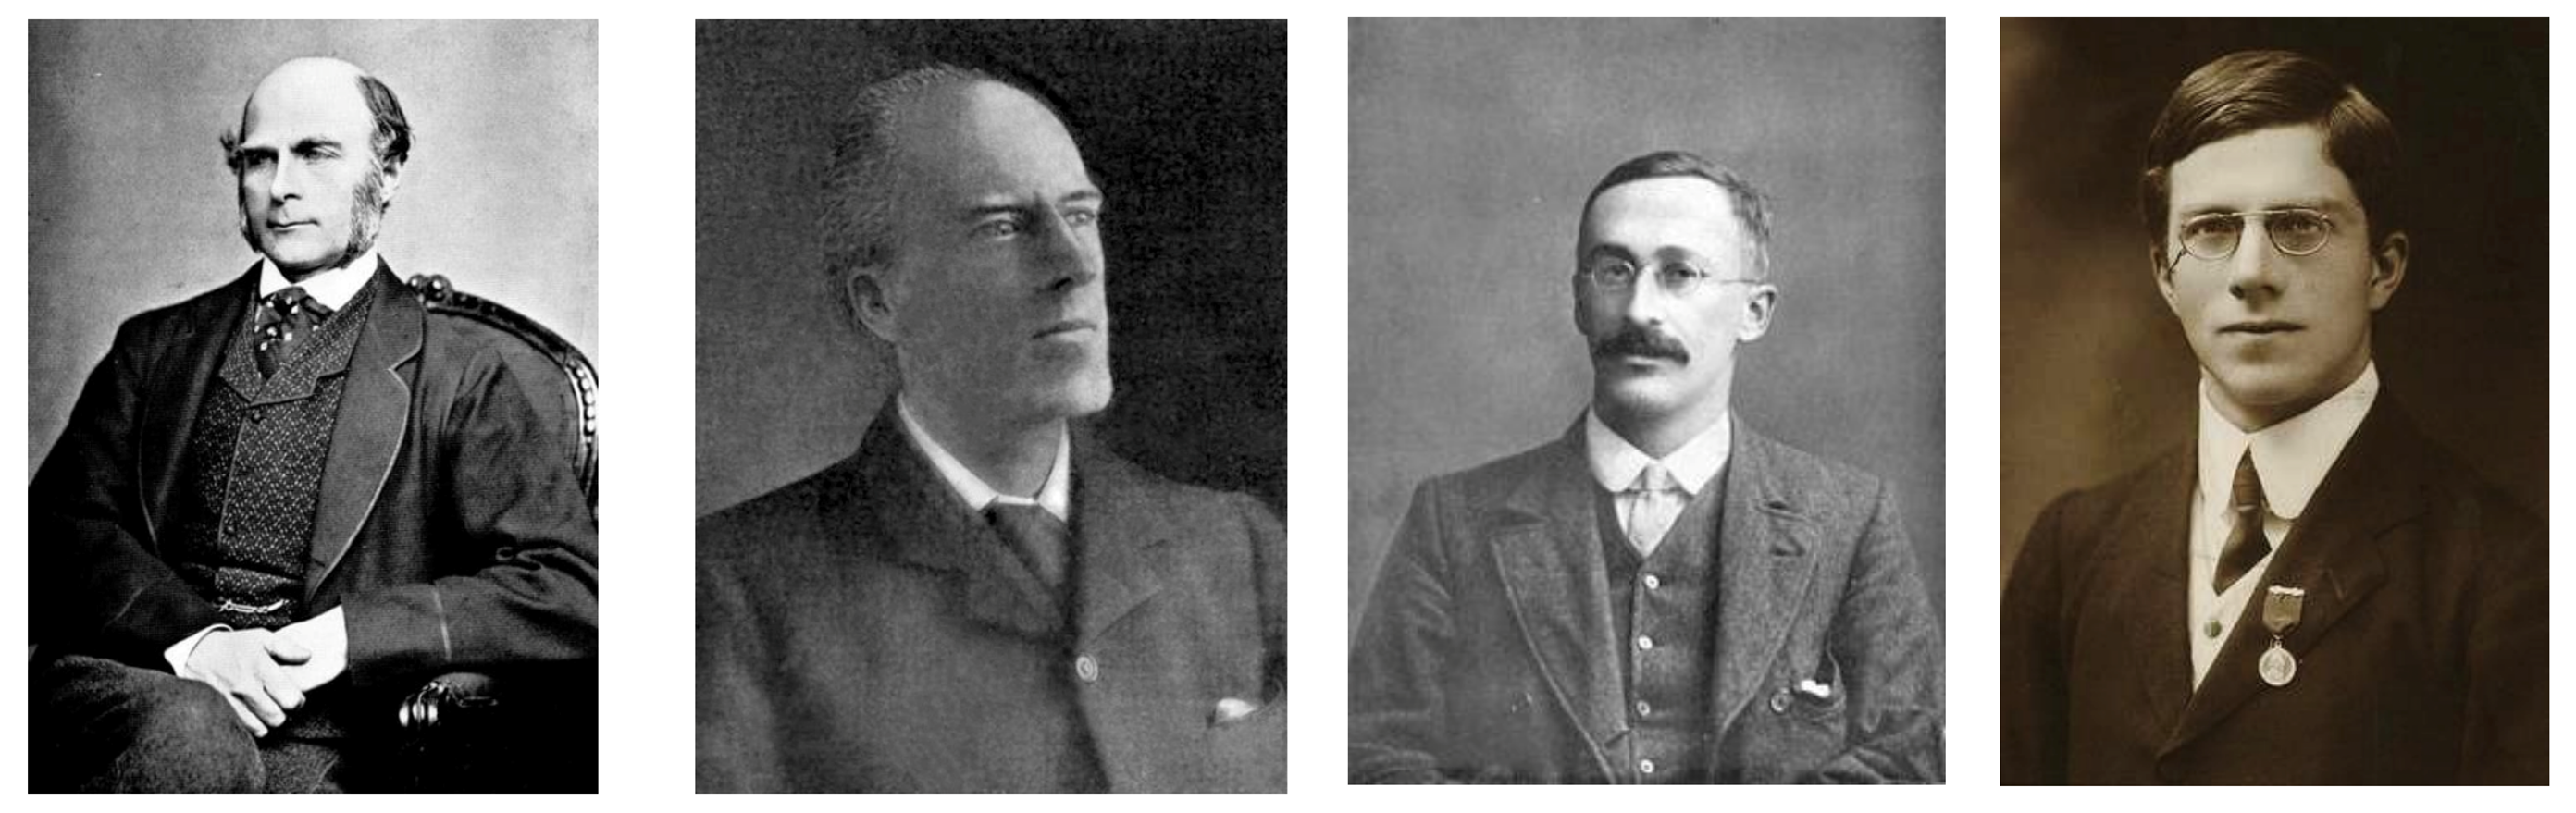
\includegraphics[width=0.9\textwidth]{figures/01-Overview/statisticians.png}
      \caption{奠基統計學的統計學家:(左至右)Francis Galton, Karl Pearson, William Gosset, Ronald Fisher}
      \label{fig:statisticians}
    \end{figure}
\chapter{資料型態與描述性統計}
    在資料分析及統計推論前,我們經常需要先對資料有初步的認識,從而決定是否要先對資料做前處理(例如轉換、合併、處理離群值等等),以及應該用什麼統計方法進行分析。當資料量不大的時候,我們可以將資料全部列出來檢視,但隨著資料量的增大,我們就需要依賴描述性統計提取資料的特徵。本章我們將認識生醫資料常見的變數型態,針對這些變數型態有哪些適用的描述性統計量和圖表,以及這些描述性統計量和圖表的基本性質。
    
    \begin{introduction}[第 \thechapter 章學習目標]
        \item 生醫資料的變數常見型態
        \item 常見的描述性統計量和圖表及適用的變數型態
        \item 資料線性轉換對平均值、變異數、標準差的影響
    \end{introduction}

\section{生醫資料中變數的常見型態}

    一般生物醫學資料最常見的格式如下表:

    \begin{table}[htbp]
        \begin{center}
            \begin{tabular}{cccccccc}
                \toprule
                年齡 & 性別 & 教育程度 & 居住地 & 身高 & 體重 & 一年癲癇發作次數 & $\cdots$\\
                \hline
                30 & 男 & 高中(職) & 北北基 & 160 & 53.3 & 3 & $\vdots$ \\
                27 & 女 & 大專 & 中彰投 & 153 & 42.6 & 0 & $\vdots$ \\
                31 & 男 & 國中以下 & 桃竹苗 & 182 & 84.2 & 2 & $\vdots$ \\
                $\vdots$ & $\vdots$ & $\vdots$ & $\vdots$ & $\vdots$ & $\vdots$ & $\vdots$ & $\vdots$ \\
                \bottomrule
            \end{tabular}
            \caption{常見資料格式\label{tab:data}}
        \end{center}
    \end{table}
        
    其中每一個 row(橫列,但不同國家的行列定義不同,因此我們這裡通稱 row)代表一筆資料,也常被稱為一個\textit{觀察值} (observation)。每個 column(直行)則代表不同的測量標的,該標的也被稱為\textit{變數}或\textit{變項} (variable)。從表\ref{tab:data}可以看出,各變項依據其可能的取值可粗略分為兩種:一種是以類別名稱取值的\textit{類別型變項} (categorical variable),例如性別、教育程度、居住地;另一種則是以有實際意義的數字取值的\textit{數值型變項} (numerical variable),例如年齡、身高、癲癇發作次數。類別型變項的各種類別取值也被稱為\textit{層次} (level)。在實務上,為了節省資料存儲空間以及減少錯誤,類別型變項的取值常會被替換為整數的數字,例如性別為男取值 1、女取值 0,或是教育程度國中以下、高中(職)、大專、碩士、博士分別替換為0、1、2、3、4。替換的數字與層次實際名稱的對照表則存儲在編碼冊 (coding book) 中,如表\ref{tab:data_coding}所示。

    \newpage

    \begin{table}[htbp]
        \begin{center}
            \begin{tabular}{cccccccc}
                \toprule
                年齡 & 性別 & 教育程度 & 居住地 & 身高 & 體重 & 一年癲癇發作次數 & $\cdots$\\
                \hline
                30 & 1 & 1 & 1 & 160 & 53.3 & 3 & $\vdots$ \\
                27 & 0 & 2 & 3 & 153 & 42.6 & 0 & $\vdots$ \\
                31 & 1 & 0 & 2 & 182 & 84.2 & 2 & $\vdots$ \\
                $\vdots$ & $\vdots$ & $\vdots$ & $\vdots$ & $\vdots$ & $\vdots$ & $\vdots$ & $\vdots$ \\
                \bottomrule
            \end{tabular}

            \bigskip

            \begin{tabular}{c|l}
                \toprule
                性別 & 女:0;男:1\\
                \hline
                教育程度 & 國中以下:0;高中(職):1;大專:2;碩士:3;博士:4\\
                \hline
                \multirow{2}{*}{居住地} & 北北基:1;桃竹苗:2;中彰投:3;\\
                & 雲嘉南:4;高屏:5;宜花東:6;外島:7\\
                \bottomrule
            \end{tabular}
            \caption{常見編碼資料格式與編碼冊\label{tab:data_coding}}
        \end{center}
    \end{table}

    根據類別型變項和數字型變項的特性,我們還可以再將它們細分:

    \begin{itemize}
        \item 類別型變項
        \begin{itemize}
            \item \textit{名目} (Nominal):各層次間沒有排序關係的類別型變項,例如性別、居住地。
            \begin{itemize}
                \item \textit{二元} (Binary):僅有兩個層次的名目變項。為了後續分析方便,通常會把其中一個層次編碼為0,另一個層次編碼為1。
                \item \textit{多元} (Multinomial):有三個以上層次的名目變項。
            \end{itemize}
            \item \textit{有序} (Ordinal):各層次間有排序關係的類別型變項,例如教育程度、收入區間。為了後續分析方便,編碼通常會按照排序關係以遞增的整數編碼,如表\ref{tab:data_coding}的教育程度編碼。
        \end{itemize}
        \item 數值型變項
        \begin{itemize}
            \item \textit{計數} (Count):取值為非負的整數,例如一年內癲癇發生次數、牙齒剩餘顆數。
            \item \textit{連續} (Continuous):實務上如果取值不連續但是可能數值足夠多(例如身高均以整數紀錄、因此可能取值有限),常常也視為連續。
            \begin{itemize}
                \item \textit{等距} (Interval):變項取值的零點是人為的,因此兩個數值相除的意義不大。例如智商、pH 值。
                \item \textit{等比} (Ratio):變項取值有一個有意義的零點,使得兩個數值相除有意義。例如身高、體重。
            \end{itemize}
        \end{itemize}
    \end{itemize}

    \begin{custom}{思考}
        根據這個定義,攝氏溫度、華氏溫度和克式溫度(Kelvin scale)應該是哪種資料型態?如果一個問卷的題目讓填答者填1到5分的(整數)滿意度,那麼這個題目的答案應該是哪種資料型態?如果疼痛指數是1到10分的整數,那麼它應該是哪種資料型態?
    \end{custom}

    \begin{custom}{思考}
        如果資料是一張 X 光片,那麼我們還能把圖像轉成數值型態嗎?更進一步,如果圖像不是黑白的,那麼要怎麼轉成數值型態?
    \end{custom}

    \begin{custom}{思考}
        一般來說,資料中的每一個 row 通常代表一筆資料,而不同的 row 通常預設是由不同的病患所貢獻。如果我們現在追蹤一群高血壓病患十年,每三個月追蹤一次(共四十次),並想記錄他們追蹤起始年齡、性別、高血壓家族史及每次追蹤的收縮壓和舒張壓,那麼應該如何記錄資料?
    \end{custom}

    了解變項的資料型態後,我們就可以進一步探討如何選擇並計算描述性統計量,來描述變項的特徵。描述性統計量本質上還是一個參數估計量(請參見第一章),而且是用來估計母體描述性參數的估計量。因此我們要先探討針對各種資料型態的母體,有哪些適用的描述性參數,以及如何用樣本計算出描述性統計量來估計這些參數。
    
\section{類別變項的描述性統計量與圖表}

    對於類別變項最具描述性的參數,即為\textit{各層次的出現比例}(由於類別變項各層次對應的編碼只是人為設定,所以一般來說,母體的描述性參數不會牽涉到這些編碼的數值。)。而估計這些比例的描述性統計量也很好計算,只要計算各層次在樣本中出現的比例即可。舉例而言,假設表\ref{tab:data}是從全台灣癲癇病患中隨機抽取 250 位所得到的資料,而我們現在關注的是「教育程度」這個變項。居住地的層次總共有五個:國中以下、高中(職)、大專、碩士、博士。因此,針對教育程度變項的母體描述性參數,即為台灣癲癇病患教育程度分別為這五個層次的比例(注意到這五個比例的總和為一,所以只要知道其中四個就可以推得最後一個)。其相對應的描述性統計量就是 250 位抽中的病患中,各類教育程度的比例。這些資訊常整理如表\ref{tab:categorical_desc},其中人數為實際觀察到的層次觀察個數,也被稱為\textit{頻率} (frequency),而比例則是這些頻率的相對大小,所以也被稱為\textit{相對頻率} (relative frequency)。

    \begin{table}[htbp]
        \begin{center}
            \begin{tabular}{lrl}
                \toprule
                \textbf{教育程度} & \textbf{人數} & \textbf{(比例\%)}\\
                \hline
                國中以下 & 52 & (20.8)\\
                高中(職) & 60 & (24.0)\\
                大專 & 112 & (44.8)\\
                碩士 & 23 & (9.2)\\
                博士 & 3 & (1.2)\\
                \bottomrule
            \end{tabular}
            \caption{類別變項的頻率與相對頻率表\label{tab:categorical_desc}}
        \end{center}
    \end{table}

    表\ref{tab:categorical_desc}也可以用圖呈現。最簡單的方法是如圖\ref{fig:barplot}的\textit{長條圖} (barplot),其中左圖是用頻率做為縱軸,右圖是用相對頻率做為縱軸,橫軸則均標示各個層次的標籤。長條圖橫軸層次順序不影響圖片的正確性,但因教育程度是有序變項,所以在圖\ref{fig:barplot}中我們採用教育程度由左而右由低到高的排列,以增加直觀性。
    
    \begin{figure}[htbp]
      \centering
      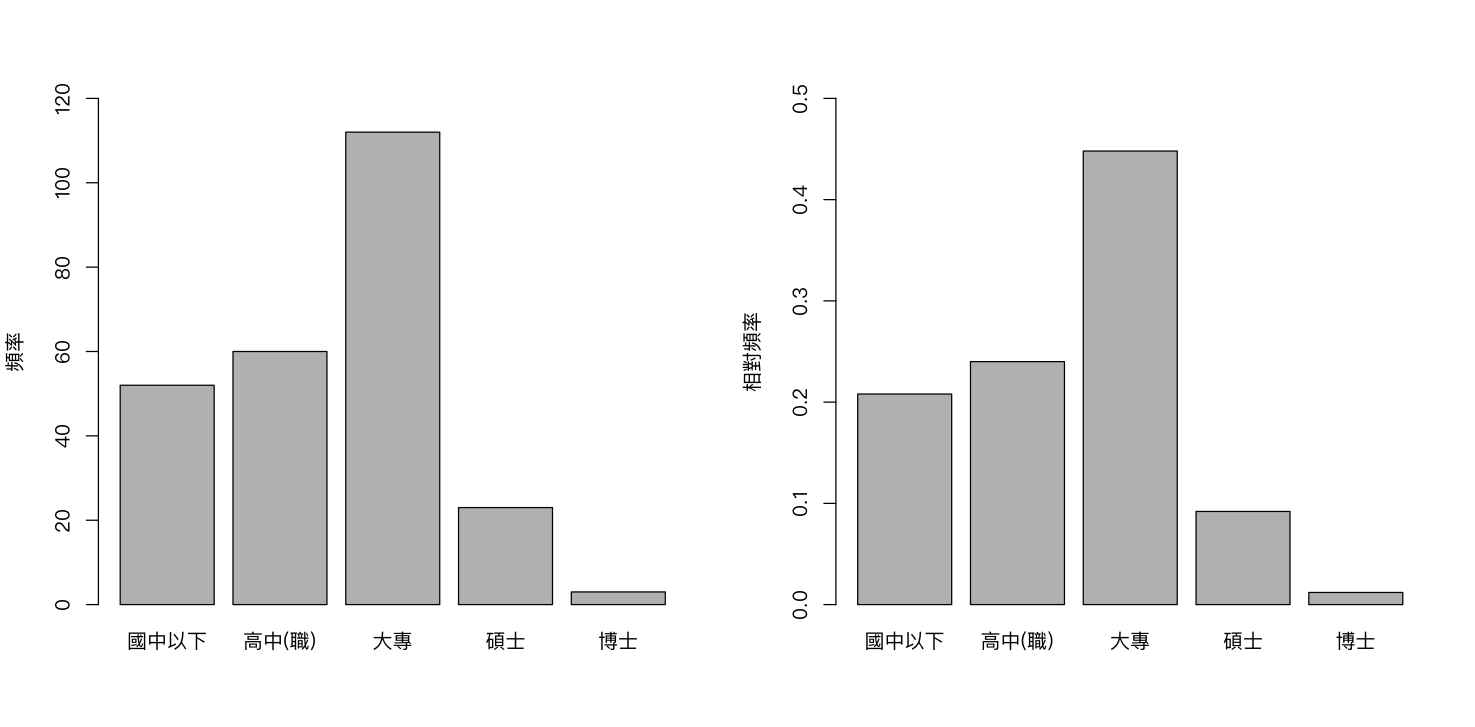
\includegraphics[width=\textwidth]{figures/02-Descriptive_statistics/barplot.png}
      \caption{以頻率與相對頻率作縱軸的長條圖}
      \label{fig:barplot}
    \end{figure}

    圖\ref{fig:pareto_chart_pie_chart}的左方是由長條圖衍生出的\textit{帕雷托圖} (Pareto chart)。其特點為層次由左而右按照頻率排列,因此靠左的層次代表佔總體的比例較大。另外,除了對應左縱軸頻率的直條圖以外,帕雷托圖還增加了一個折線圖,對應到右縱軸的\textit{累積比例} (cumulative percentage)。累積比例代表該層次及其左側的所有層次的總比例,例如國中以下的累積比例為大專的比例44.8\% + 高中(職)的比例 24.0\% + 國中以下的比例 20.8\%,總和為 89.6\%。繪製累積比例的好處在於,讀者可以輕易看出該變項是否主要由特定一群層次所組成,以及其所佔比例,例如大專和高中(職)畢業的病患大約佔了總體 70\%。圖\ref{fig:pareto_chart_pie_chart}的右方則是常見的\textit{圓餅圖} (pie chart)。除非層次的佔比很懸殊,否則圓餅圖很難直觀表現出層次佔比的差異(例如國中以下和高中(職)的佔比大小,單就圖而言很難分出來),所以通常不建議使用。\;\;\;\;\;\;\phantom{X}

    \begin{figure}[htbp]
      \centering
      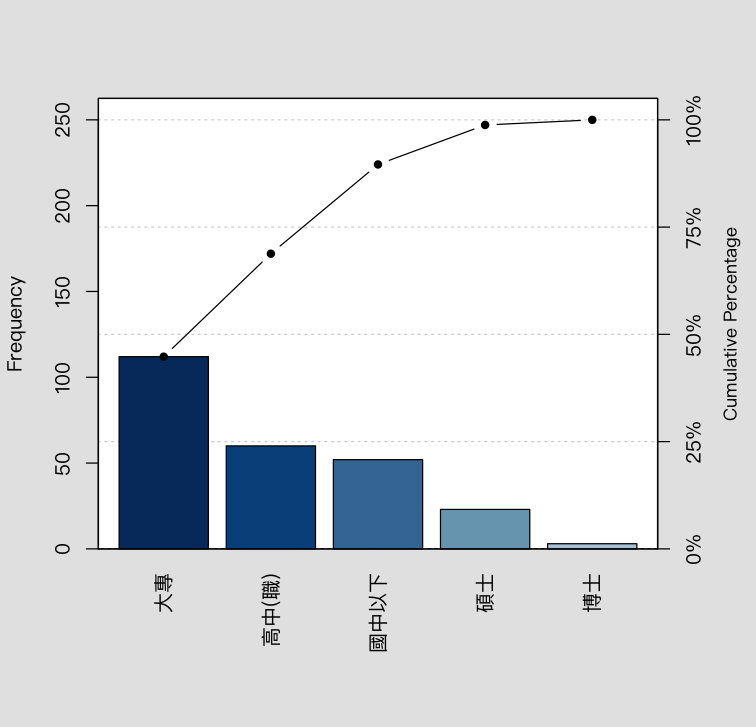
\includegraphics[width=0.48\textwidth]{figures/02-Descriptive_statistics/pareto_chart.png}
      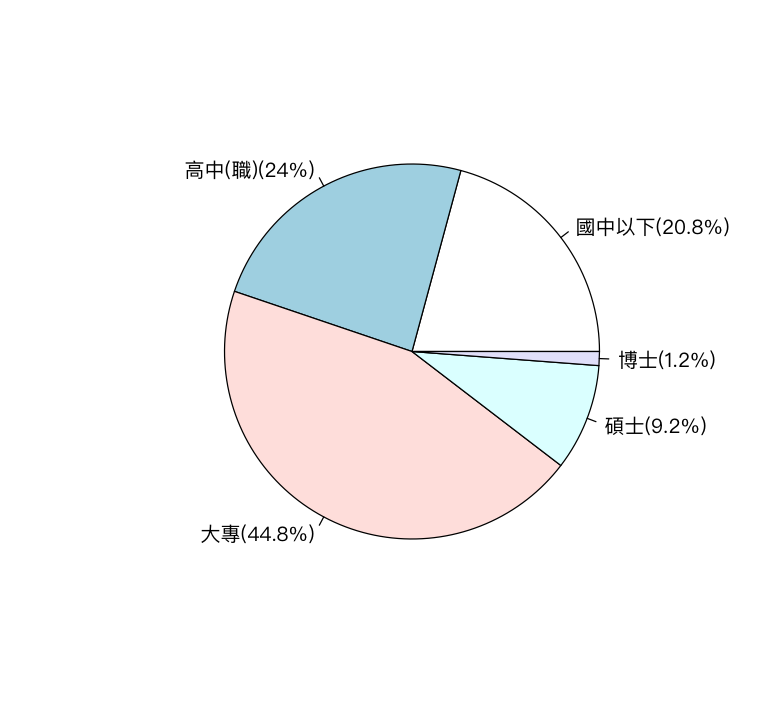
\includegraphics[width=0.48\textwidth]{figures/02-Descriptive_statistics/pie_chart.png}
      \caption{帕雷托圖與圓餅圖}
      \label{fig:pareto_chart_pie_chart}
    \end{figure}
    
    %我們從清華大學隨機抽取了 100 位大學生並記錄了「性別」這個變項。我們的母體是清華大學的所有大學生,而這些大學生的性別層次有兩個:男和女,所以針對性別變項的母體描述性參數即為「清華大學生的男生比例」及「清華大學生的女生比例」(因為加起來等於一,所以知道一個比例就可以推出另外一個)。相對應的描述性統計量就是 100 位抽中的大學生中,男性和女性的比例。

\section{數值變項的描述性統計量及圖表}
    和類別變項不同的是,數值變項的取值可能性多了許多,而且具有解釋意義。因此數值變項的母體描述性參數相對於類別變項更為多元。針對數值變項,我們能用\textit{直方圖} (histogram) 來視覺化母體的取值狀況,如圖\ref{fig:descriptive_cont}所示。繪製直方圖時,我們先將數值變項依可能取值切割成大小相等的區間,例如圖\ref{fig:descriptive_cont}中我們把取值區間以 0.5 的寬度分成$[10,10.5),[10.5,11),[11,11.5),...,[19.5,20)$,其中 $[a,b)$ 代表 $\ge a$ 但 $<b$ 的區間。而後即可計算落入各區間的觀察值個數並以直條繪製頻率或相對頻率。注意到直方圖和長條圖不同地方在於,直方圖的每個直條之間是\textbf{沒有}間隙的(除非有區間恰好沒有觀察值)、而且不能隨意交換順序,以表明直方圖的各直條代表連續且有序的組別。

    \bigskip
    
    \begin{custom}{思考}
        在製作直方圖時,如果區間寬度過大或過小,會對圖造成什麼影響?
    \end{custom}

    \bigskip

    \begin{figure}[htbp]
      \centering
      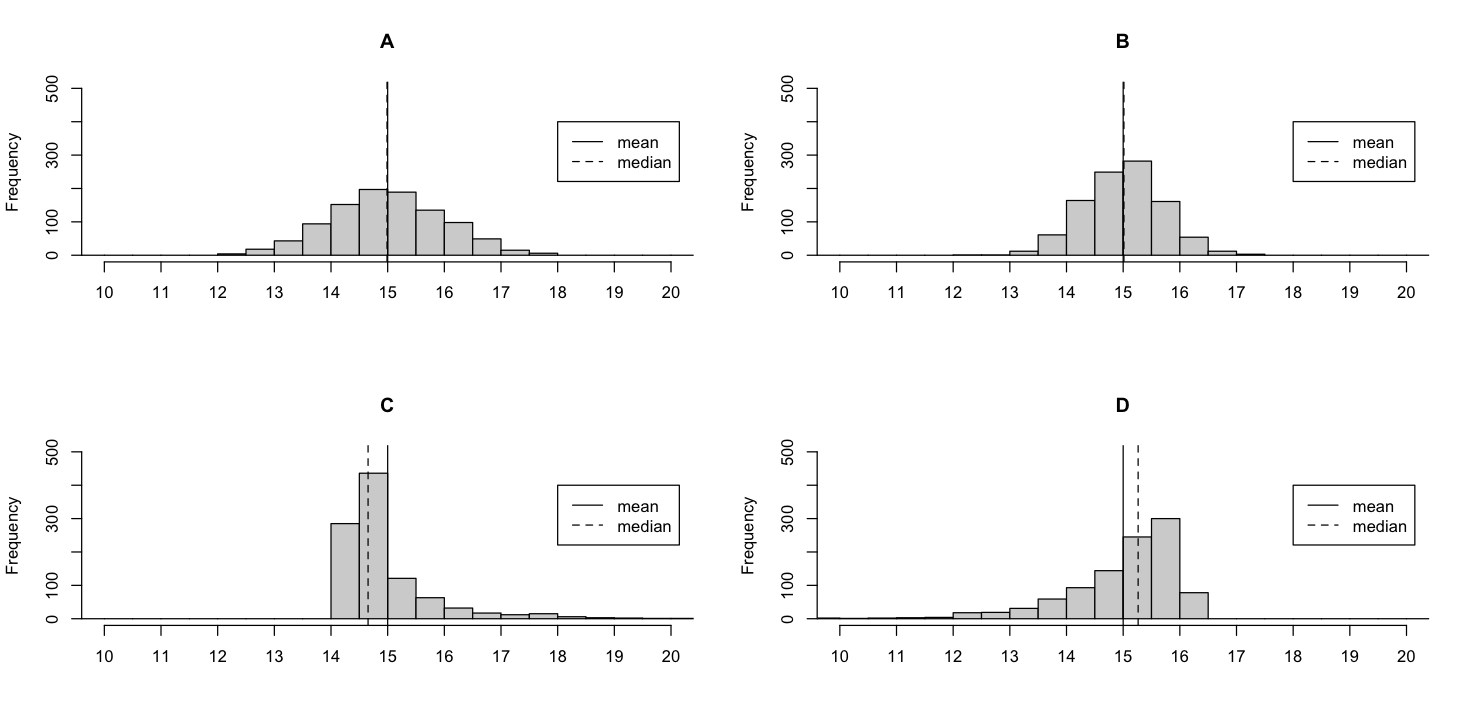
\includegraphics[width=\textwidth]{figures/02-Descriptive_statistics/descriptive_cont.png}
      \caption{四個不同母體的分布直方圖}
      \label{fig:descriptive_cont}
    \end{figure}

    \bigskip
        
    以下我們根據圖\ref{fig:descriptive_cont}討論一些常用的描述性參數。

\subsection{位置參數及其描述統計量}
    描述變項母體分佈的第一步,通常是找尋它的中心位置,我們才知道可能的取值大多會落在哪個數值附近。描述母體中心位置的參數通常被稱謂\textit{位置參數} (location parameter)。其中最常見的位置參數就是我們耳熟能詳的\textit{平均值} (mean),或是更精準的一點說,\textit{算術平均值} (population arithmetic mean)。假設變項 $X$ 的母體有 $N$ 個觀察值,分別為 $\tilde{X}_1, \tilde{X}_2, ... \tilde{X}_N$,則 $X$ 的\textit{母體平均} $\mu_X$ 的定義為:
    \[\mu_X = \frac{\tilde{X}_1+\tilde{X}_2+\cdots+\tilde{X}_N}{N} = \frac{1}{N}\sum_{i=1}^N \tilde{X}_i\]
    估計母體平均值的描述統計量被稱為\textit{樣本平均} (sample mean),常簡寫為 $\bar{X}$(唸作 X bar),假設樣本數為 $n$,觀察值分別為$X_1, X_2, ... X_n$,則樣本平均 $\bar{X}$ 的定義很直觀:
    \[\bar{X} = \frac{X_1+X_2+\cdots+X_n}{n} = \frac{1}{n}\sum_{i=1}^n X_i\]
    也就是把樣本觀察值全部加總取平均。注意到如果把變項做線性的放大平移 $X^* = aX+b$ ,也就是將放大$a$倍後加上$b$,那麼新的母體平均和樣本平均 $\mu_X^*$ 和 $s_X^2$ 會變成:
    \begin{align*}
        \mu_X^* &= \frac{(a\tilde{X}_1+b)+(a\tilde{X}_2+b)+\cdots+(a\tilde{X}_N+b)}{N}\\
        &= \frac{a(\tilde{X}_1+\tilde{X}_2+\cdots+\tilde{X}_N)+Nb}{N}\\
        &= a\frac{\tilde{X}_1+\tilde{X}_2+\cdots+\tilde{X}_N}{N} + \frac{Nb}{N} = a\mu_X + b\\
        \bar{X}^* &= \frac{(aX_1+b)+(aX_2+b)+\cdots+(aX_n+b)}{n}\\
        &= \frac{a(X_1+X_2+\cdots+X_n)+nb}{n}\\
        &= a\frac{X_1+X_2+\cdots+X_n}{n}+\frac{nb}{n}=a\bar{X}+b
    \end{align*}
    所以平均值同樣會以相同的倍率放大平移。
    
    平均值的算法雖然簡單,但是它的數值很容易受到極端的觀察值影響而偏移。例如在圖\ref{fig:descriptive_cont}的 C 中,雖然大於七成的母體取值都落在 14 到 15 之間,但母體平均值受到右方較大的數值影響而被往右拉到 15。此處以平均值 15 當作母體分布的「中心」似乎就不太合理。\textit{中位數} (median)是解決這個問題的一個替代方案,它的想法是把所有的取值由小排到大,並選取位置在正中間的數值。如果取值的數目為偶數,則取最中間兩個數值的平均。換句話說,如果把變項 $X$ 的母體觀察值由小排到大得到 $\tilde{X}_{(1)}, \tilde{X}_{(2)}, ..., \tilde{X}_{(N)}$,則母體中位數 $M_X$ 的定義為:
    \[M_X = \left\{\begin{array}{lr}
        \tilde{X}_{(\frac{N+1}{2})}, & N \text{是奇數}\\
        \frac{1}{2}\Big[\tilde{X}_{(\frac{N}{2})}+\tilde{X}_{(\frac{N}{2}+1)}\Big], & N \text{是偶數}
    \end{array}\right.\]
    估計母體中位數的描述性統計量即為\textit{樣本中位數} (sample median),其定義一樣很直觀:假設樣本觀察值由小排到大分別為$X_{(1)}, X_{(2)}, ... X_{(n)}$,則樣本中位數 $\hat{M}_X$ 為:
    \[\hat{M}_X = \left\{\begin{array}{lr}
        X_{(\frac{N+1}{2})}, & N \text{是奇數}\\
        \frac{1}{2}\Big[X_{(\frac{N}{2})}+X_{(\frac{N}{2}+1)}\Big], & N \text{是偶數}
    \end{array}\right.\]
    如前所述,中位數雖然常和平均值相去不遠,但是當變項的分布在一個方向有較多的極端值時,中位數就會和平均值有差距。如果極端值較常出現在右側,我們稱該分布為\textit{右偏} (right-skewed)或\textit{正偏} (positively skewed),此時一般而言,中位數會比平均值來得小(如圖\ref{fig:descriptive_cont}的C)。反之,如果極端值較常出現在左側,我們稱該分布為\textit{左偏} (left-skewed)或\textit{負偏} (negatively skewed),此時一般而言,中位數會比平均值來得大(如圖\ref{fig:descriptive_cont}的D)。
    
    雖然中位數雖然的確能夠直指分布的「中心」,但它的統計性質較為複雜,在後續很多的推論統計方法沒有辦法直接適用,因此一般而言我們還是會優先選擇平均值作為我們的位置參數以及描述統計量。另外一個可用的位置參數是 \textit{眾數} (mode),也就是所有觀察值中出現頻率最高的數值。不過在數值型變項,尤其是連續型變項中,各樣本取值的頻率常常都很低(例如一群人中,體重數值如果取到小數點後一位,那麼每種可能取值的出現次數可能都只有一次),所以實務上不常使用。

    \bigskip
    
    \begin{custom}{思考}
        如果某個變項在收集的過程中,已經先行將連續的變項分割為多個區間,並且記錄區間的頻率(例如 10-20 歲多少人、20-30 歲多少人、40-50 歲多少人),那麼我們還有辦法對該變項計算位置相關的描述統計量嗎?
    \end{custom}

\subsection{分散參數及其描述統計量}
    除了位置參數以外,我們看到 A 和 B 兩個變項的母體平均值和中位數均為 15 ,但是 B 的可能取值跨度明顯地比 A 還要小。換句話說,相對於 A,B 的取值比較常落在離平均值比較近的位置。用來描述這個分布特性的參數稱為分散參數 (dispersion parameter)。
    
    一個變項的取值和平均值之間的距離,如果平均而言較遠(例如圖\ref{fig:descriptive_cont}中的 A 有為數不少的取值跟平均值 15 的距離大於 1),那麼這個變項的分散程度應該比較大。因此,直覺上分散參數的定義可以用「取值和平均值的平均距離」來定義。如此定義的分散參數稱為\textit{平均絕對離差} (mean absolute deviation),也就是:
    \[\text{MAD}_X = \frac{|\tilde{X}_1-\mu_X|+|\tilde{X}_2-\mu_X|+\cdots+|\tilde{X}_N-\mu_X|}{N} = \frac{1}{N} \sum_{i=1}^N |\tilde{X}_i-\mu_X|\]

    雖然平均絕對離差的定義很符合直覺,但是它含有絕對值,處理起來較為複雜。因此,統計學中較常使用的分散參數定義為「取值和平均值之平方距離的平均」。如此定義的分散參數即為著名的\textit{變異數} (variance),通常記為$\sigma^2_X$。以符號定義母體變異數 (population variance) 如下:
    \[\sigma^2_X = \frac{(\tilde{X}_1-\mu_X)^2+(\tilde{X}_2-\mu_X)^2+\cdots+(\tilde{X}_N-\mu_X)^2}{N} = \frac{1}{N} \sum_{i=1}^N (\tilde{X}_i-\mu_X)^2\]
    估計母體變異數的描述性統計量稱為\textit{樣本變異數} (sample variance),通常以 $s^2_X$ 代表。按照前面平均值和中位數的經驗,樣本變異數應該直接把母體觀察值 $\tilde{X}_i$ 換成樣本觀察值 $X_i$。但是這樣還不夠,因為我們不知道母體平均數 $\mu_X$ 的值,所以需要用樣本平均數 $\bar{X}$ 來估計代換 $\mu_X$,而得到下面的式子:
    \[\frac{(X_1-\bar{X})^2+(X_2-\bar{X})^2+\cdots+(X_n-\bar{X})^2}{n}\]
    很不幸地,上述的樣本估計式會\textbf{低估}母體變異數。我們可以用圖\ref{fig:degrees_of_freedom}來獲得一個直覺的解釋。當我們抽樣都抽到數值較小的觀察值時(如圖\ref{fig:degrees_of_freedom}中的四個紅點),母體變異數的定義希望我們計算觀察值到\textbf{母體平均}的平方距離,此時母體平均比樣本觀察值都來得大(圖\ref{fig:degrees_of_freedom}的實線),但是這個估計式是計算觀察值到\textbf{樣本平均}的平方距離,而樣本平均基本上會在樣本觀察值的中心(圖\ref{fig:degrees_of_freedom}的虛線)。因此,估計式計算出的平方距離會比母體變異數想要計算的來得小。同樣的,如果抽樣都抽到數值較大的觀察值,也是會有低估的狀況。解決的方法是對分母做一個校正:除以樣本數減一($n-1$)而不是樣本數。至於為何是樣本數減一而不是減其他數,我們會在後續的課程做說明,這裡就暫且假設下述的定義是較佳的樣本變異數計算方法:
    \[s^2_X = \frac{(X_1-\bar{X})^2+(X_2-\bar{X})^2+\cdots+(X_n-\bar{X})^2}{n-1} = \frac{1}{n-1} \sum_{i=1}^n (X_i-\bar{X})^2\]

    \begin{figure}[htbp]
      \centering
      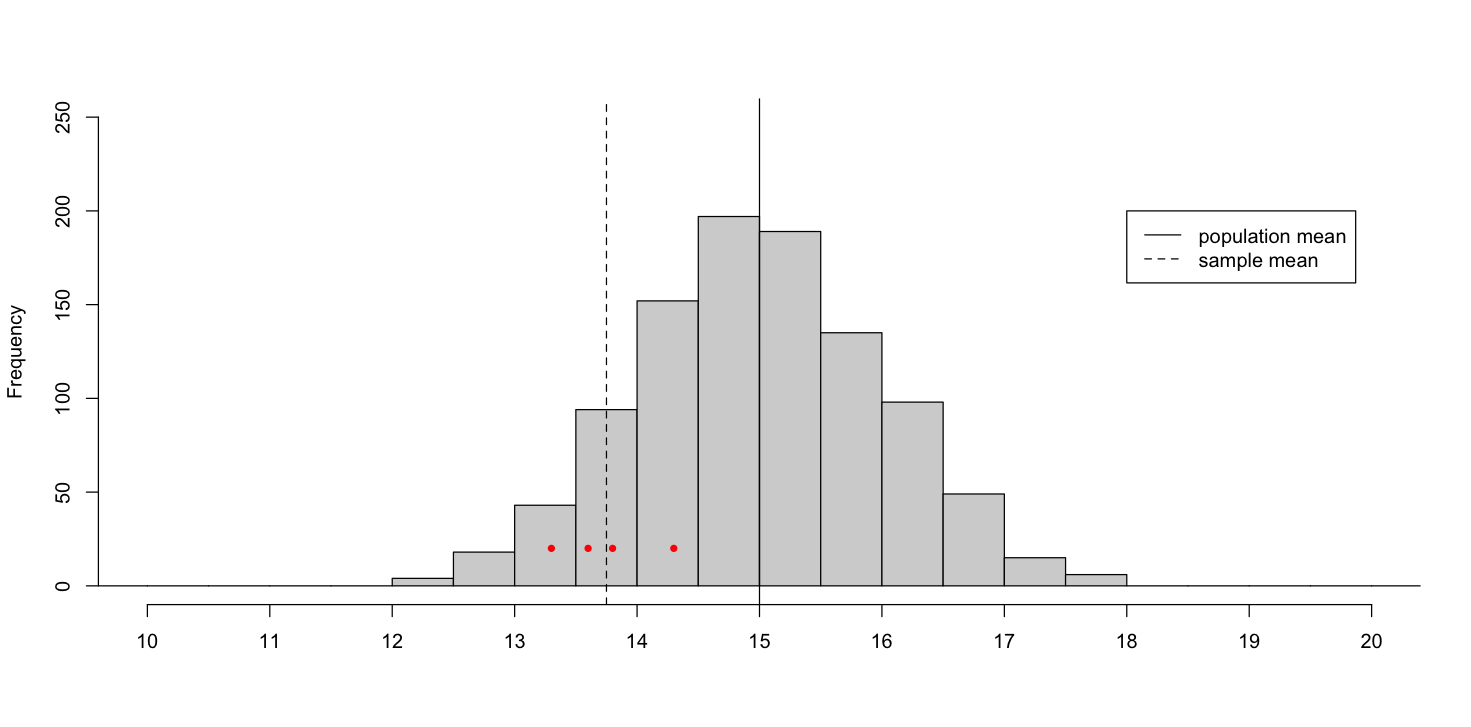
\includegraphics[width=\textwidth]{figures/02-Descriptive_statistics/degrees_of_freedom.png}
      \caption{估計母體變異數的低估問題}
      \label{fig:degrees_of_freedom}
    \end{figure}

    變異數雖然是一個很好用的分散參數,但如果仔細思考它的定義,會發現因為它是對「取值和母體平均之差值」的平方取平均,所以變異數的單位會是該變項單位的平方。例如,如果變項是收縮壓,單位是mmHg,那麼變異數的單位就會是$\text{mmHg}^2$,造成我們解釋上的困難(想像如何解釋 $100\text{mmHg}^2$!)。因此,我們再定義一個變異數的開根號為\textit{標準差} (standard deviation),作為一個新的分散參數。母體標準差通常寫作$\sigma_X$,其符號定義如下:
    \[\sigma_X = \sqrt{\frac{(\tilde{X}_1-\mu_X)^2+(\tilde{X}_2-\mu_X)^2+\cdots+(\tilde{X}_N-\mu_X)^2}{N}} = \sqrt{\frac{1}{N} \sum_{i=1}^N (\tilde{X}_i-\mu_X)^2}\]
    而估計母體標準差的樣本估計量稱為樣本標準差,通常記做$s$,其符號定義也十分直覺:
    \[s_X = \sqrt{\frac{(X_1-\bar{X})^2+(X_2-\bar{X})^2+\cdots+(X_n-\bar{X})^2}{n-1}} = \sqrt{\frac{1}{n-1} \sum_{i=1}^n (X_i-\bar{X})^2}\]
    (註:理論上上述的樣本標準差還要再進行校正才會成為母體標準差的最佳估計方法,但實務上差異不大且太過複雜,所以大多使用上述的簡單公式。)

    標準差的單位和原變項相同,因此可以看成是分布「寬度」的一個指標。若將其與平均值的組合,可以讓我們對變項做最初步的了解。在母體分布不要太奇形怪狀的情況下,我們可以套用經驗性的「68-95-99.7法則」:
    \begin{itemize}
        \item 母體約有$68\%$的取值會在 $\mu-\sigma$ 與 $\mu+\sigma$ 之間
        \item 母體約有$95\%$的取值會在 $\mu-2\sigma$ 與 $\mu+2\sigma$ 之間
        \item 母體約有$99.7\%$的取值會在 $\mu-3\sigma$ 與 $\mu+3\sigma$ 之間
    \end{itemize}
    因此,如果資料中出現離平均值兩倍標準差、甚至三倍標準差以外的觀察值,就可以進一步調查該觀察值,是否有測量錯誤的問題。
    
    如同之前在平均值的討論,我們也可以探討變項如果做線性的放大平移,會對變異數和標準差造成什麼影響。首先,直覺上,因為平移變項的數值並不會改變其分散程度,所以平移不應該改變變異數及標準差。我們可以簡單地驗證:假設我們對變項 $X$ 做平移得到 $X^* = X+b$,則我們已知母體平均數會變成 $\mu_X^* = \mu_X+b$,所以新的母體變異數為:
    \begin{align*}
        \sigma^{2*}_X &= \frac{[(\tilde{X}_1+b)-(\mu_X+b)]^2+[(\tilde{X}_2+b)-(\mu_X+b)]^2+\cdots+[(\tilde{X}_N+b)-(\mu_X+b)]^2}{N} \\
        &= \frac{[\tilde{X}_1-\mu_X]^2+[\tilde{X}_2-\mu_X]^2+\cdots+[\tilde{X}_N-\mu_X]^2}{N} = \sigma_X^2
    \end{align*}
    同樣地,樣本變異數也不會受到平移的影響。由於標準差為變異數開根號,所以也不會受到平移的影響。

    假設我們並非對變項 $X$ 做平移,而是縮放而得到 $X^* = aX$,例如把 $X$ 的測量單位從公尺變成公分,使得數值變為 100 倍,則我們已知母體平均數會變成 $\mu_X^* = a\mu_X$,所以新的母體變異數為:
    \begin{align*}
        \sigma^{2*}_X &= \frac{(a\tilde{X}_1-a\mu_X)^2+(a\tilde{X}_2-a\mu_X)^2+\cdots+(a\tilde{X}_N-a\mu_X)^2}{N} \\
        &= a^2\frac{(\tilde{X}_1-\mu_X)^2+(\tilde{X}_2-\mu_X)^2+\cdots+(\tilde{X}_N-\mu_X)^2}{N} = a^2\sigma_X^2
    \end{align*}
    因此,縮放後,母體變異數會以平方的倍數被縮放。同樣地,樣本變異數也會被平方的倍數縮放。由於標準差為變異數開根號,所以標準差的縮放倍數會和變項的縮放倍數大小相同(需加上絕對值),也就是$\sigma^*_X = |a|\sigma_X$。

    除了變異數和標準差外,\textit{全距} (range) 和 \textit{四分位差} (interquartile range, IQR) (尤其是四分位差)也會被拿來作為量化變數分散程度的描述統計量。全距的定義十分直觀,即為最大觀察值和最小觀察值之差,不過也因此全距非常容易受到極端值的影響,對於分散程度的量化效果不如其他統計量。四分位差則牽涉到百分位數的計算。我們之前計算過的中位數其實就是第 $50$ 百分位數,而第 $p$ 百分位數的計算方式為($\lceil.\rceil$為取比括號內大的最小整數)
    \[\left\{\begin{array}{lr}
        X_{(\lceil np/100 \rceil)}, & np/100 \text{非整數}\\
        \frac{1}{2}\Big[X_{(np/100)}+X_{(np/100+1)}\Big], & np/100 \text{為整數}
    \end{array}\right.\]
    第一、第二、第三四分位分別為變項的第 25、50、75 百分位數,而四分位差的定義則為第三四分位與第一四分位的差。由此可以看到,四分位差不會受到數值最大和最小 25$\%$ 資料的影響,對於極端值較不敏感。因此在實務上,如果資料分布有較多的極端值,如圖\ref{fig:descriptive_cont}中的C和D,可以考慮以四分位差取代標準差作為分散程度的指標。

    \bigskip

    \begin{custom}{思考}
        如果對資料作線性的放大平移,那麼中位數、全距和四分位差應該會如何變動?
    \end{custom}

\subsection{數值變項的描述性統計圖表}
    除了前面提到的直方圖外,另一種常用來描述連續變項分布的圖表是\textit{盒形圖} (boxplot) 或\textit{盒鬚圖} (box-and-whisker plot),如圖\ref{fig:boxplot_stem}的左圖。盒鬚圖的好處是可以在有限的空間中描繪資料的中心、分散度、偏度以及可能的\textit{離群值} (outlier)。盒鬚圖分成三部分:盒子、鬍鬚和代表離群值的圓點。盒子的部分代表變項取值的主要範圍,上下分別為變項的第三四分位 (Q3) 和第一四分位 (Q1),而中間的線段代表中位數 (M)。圓點的部分代表離群值,常見的離群值定義以四分位差 (IQR) 作為分散程度的標準:取值若落在 Q3 + 1.5 IQR 以及 Q1 - 1.5 IQR 以外,則標記為離群值。最後鬍鬚的部分則畫出非離群值之取值範圍,因此上限(U)為不大於 Q3 + 1.5 IQR 的最大觀察值,而下限(L)為不小於 Q1 - 1.5 IQR 的最小觀察值。盒鬚圖中間的小菱形並非必要,若有畫上則通常代表平均值。

    在直方圖中,每個直條僅能說明在該區間中有多少觀察值,但觀察值在區間內的分布則無從得知。當資料量比較少時,\textit{莖葉圖} (stem-and-leaf plot)可以提供比直方圖更多的資訊。在莖葉圖中,所有的觀察值都被拆成兩部分:左邊帶頭的一串數字(莖)以及最右邊的一位數字(葉)。例如 4, 10, 81 被分為 (0,4), (1,0), (8,1)。而後先把最小的莖安置在左上角,並依序向下加一至最大的莖。而後將每個觀察值的葉,按照其莖的位置,排序填入莖的右側,即可得到如圖\ref{fig:boxplot_stem}之右圖的莖葉圖。可以看到,莖葉圖保有直方圖的特性:每一個莖右邊的葉子長度即為該代表區間的觀察值數,例如落在 [40,50) 的觀察值僅有兩個。另外,在每個莖中,可以依據右邊葉子數字的分布,了解區間內資料的分布狀況。例如在 [10, 20) 這個區間中,葉的數值大多集中在小數字,也就是在這個區間中分布是比較右偏的。

    \begin{figure}[htbp]
        \centering
        \begin{minipage}{.5\textwidth}
            \centering
            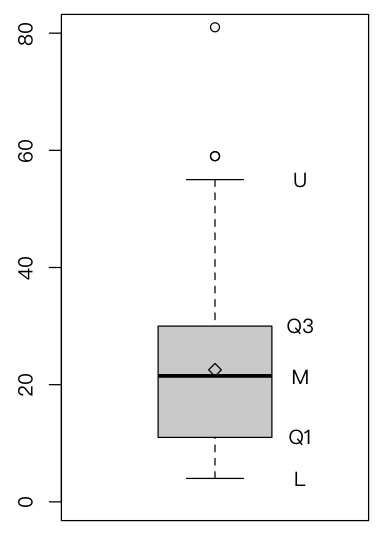
\includegraphics[width=0.9\textwidth]{figures/02-Descriptive_statistics/boxplot.png}
        \end{minipage}%
        \begin{minipage}{.5\textwidth}
            \centering
            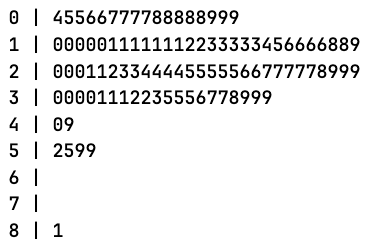
\includegraphics[width=0.9\textwidth]{figures/02-Descriptive_statistics/stem_and_leaf.png}
        \end{minipage}
        \caption{盒鬚圖與莖葉圖}
        \label{fig:boxplot_stem}
    \end{figure}

    \bigskip

    \begin{custom}{思考}
        直方圖和盒鬚圖各自提供了哪些對方所沒有的資訊?是否有可能將兩者合併?
    \end{custom}

    \begin{docexam}{(104-1醫學(一))}
        下列那個測量值較不易受到資料極端值的影響?
        
        (A) 平均值  (B) 中位數  (C) 全距  (D) 標準差
    \end{docexam}

    \begin{docexam}{(102-1醫學(一))}
        下列何種統計指標較不受極端值的影響?
        
        (A) 平均值  (B) 第75百分位數  (C) 樣本標準差  (D) 樣本標準誤
    \end{docexam}

    \begin{docexam}{(102-1醫學(一))}
        下列資料是 6 隻長有癌細胞老鼠,經過放射線治療後的存活時間(月):1.4, 1.7, 2.3, 2.5, 3.2, 3.8。如果 3.8 這筆資料在紀錄時,被錯誤地記為 38,下列哪一個敘述隊統計量的影響是正確的?
        
        (A) 中位數增加  (B) 眾數增加  (C) 平均值增加  (D) 中位數和平均值同時增加
    \end{docexam}

    \begin{docexam}{(101-1醫學(一))}
        下列資料代表 6 個接受髖關節置換手術病人的住院天數(天):4, 3, 3, 5, 4, 20,哪一個集中趨勢統計量最適合描述此資料?
        
        (A) 平均值  (B) 全距  (C) 眾數  (D) 中位數
    \end{docexam}

    \begin{docexam}{(100-2醫學(一))}
        有一位研究者想瞭解抽菸和肥胖間的相關,肥胖程度用身體質量指數測量,身體質量指數(BMI)=體重(公斤)/身高$^2$(公尺),此研究者想描述抽菸者和非抽菸者的BMI集中趨勢,下列何者統計量最適合?
        
        (A) 平均值  (B) 全距  (C) 百分比  (D) 眾數
    \end{docexam}

    \begin{docexam}{(109-1醫學(二))}
        有關描述變項的性質,下列敘述何者正確?
        
        (A) 標準誤 (standard error) 適合描述常態連續資料的分散情況
        
        (B) 幾何平均值 (geometric mean) 適合描述類別資料的集中趨勢
        
        (C) 標準差 (standard deviation) 適合描述類別資料的集中趨勢
        
        (D) 第 50 百分位數 (the 50th percentile) 適合描述連續資料的集中趨勢
    \end{docexam}

    \begin{docexam}{(108-1醫學(二))}
        關於測量尺度(measurement scale)的敘述,下列何者正確?
        
        (A) 血型為序位尺度 (ordinal scale)
        
        (B) 膽固醇值 (mg/100ml) 為等比尺度 (ratio scale) 
        
        (C) 體溫 (攝氏度 C) 為等比尺度 (ratio scale)
        
        (D) 癌症分期為等距尺度 (interval scale)
    \end{docexam}

\nocite{*} 
% \appendix
% \chapter{線性代數}

\section{線性代數}

\subsection{橫向量、縱向量}
線性代數,而且能讓。

橫向量(row vector, 大陸稱為行向量、台灣稱為列向量)
\[\begin{bmatrix} 1 & 2 & 3 \end{bmatrix}\]

縱向量(column vector, 大陸稱為列向量、台灣稱為行向量)
\[\begin{bmatrix} 
    1 \\ 
    2 \\ 
    3 
  \end{bmatrix}\]
    
向量內積
\[\begin{bmatrix} 
    u_1 & u_2 & \cdots & u_k 
  \end{bmatrix}\begin{bmatrix} 
    v_1 \\
    v_2 \\
    \vdots \\
    v_k 
  \end{bmatrix} = u_1v_1 + u_2v_2 + \cdots + u_kv_k\]
  
向量外積
\[\begin{bmatrix} 
    u_1 \\
    u_2 \\
    \vdots \\
    u_k 
  \end{bmatrix}\begin{bmatrix} 
    v_1 & v_2 & \cdots & v_k 
  \end{bmatrix} = \begin{bmatrix}
    u_1v_1 & u_1v_2 & \cdots & u_1v_k\\
    u_2v_1 & u_2v_2 & \cdots & u_2v_k\\
    \vdots & \vdots & \ddots & \vdots\\
    u_kv_1 & u_kv_2 & \cdots & u_kv_k\end{bmatrix}\]

\begin{note}
haha
\end{note}

% \bibliography{reference}

\end{document}
